% Created 2020-02-10 Mon 22:57
% Intended LaTeX compiler: pdflatex
\documentclass[bigger]{beamer}
\usepackage[utf8]{inputenc}
\usepackage[T1]{fontenc}
\usepackage{graphicx}
\usepackage{grffile}
\usepackage{longtable}
\usepackage{wrapfig}
\usepackage{rotating}
\usepackage[normalem]{ulem}
\usepackage{amsmath}
\usepackage{textcomp}
\usepackage{amssymb}
\usepackage{capt-of}
\usepackage{hyperref}
\usepackage{comment}
\usetheme{Hannover}
\author{Ben Lewis}
\date{\today}
\title{Beyond Two Cans and a String}
\subtitle{A practical guide to building a router}
\hypersetup{
 pdfauthor={Ben Lewis},
 pdftitle={Beyond Two Cans and a String},
 pdfkeywords={},
 pdfsubject={Broaden your homelab experiments to include your network fabric itself, have fun, and learn something along the way as we talk about what choices you can make in building your own home router.},
 pdfcreator={Emacs 26.3 (Org mode 9.1.9)}, 
 pdflang={English}}
\excludecomment{notes}
\begin{document}

\maketitle
\begin{frame}{Outline}
\tableofcontents
\end{frame}


\section{Consumer routers bore me}
\label{sec:org769d52d}

\subsection{Background}
\label{sec:orgb37081c}

\begin{frame}[fragile,label={sec:org06c16c6}]{\texttt{whoami}}
  \begin{itemize}
  \item Software engineer by day
  \item I care too much about RFCs
  \item In my spare time, I work on my hackerspace's network.
  \end{itemize}
\begin{notes}
I'm an unabashed text console enthusiast. I like to manage my equipment via
command lines and SSH; it means I have a uniform interface when dealing with
machines all over the place, and I can use it from pretty much anywhere-even my
phone.

But command line interfaces just aren't common on most consumer equipment sold
today, in fact, they basically don't exist. That's a huge bummer for me, and
caused me to start looking for other options.
\end{notes}

\end{frame}

\subsection{Limitations of consumer hardware}
\label{sec:orgbbeeef6}

\begin{frame}[label={sec:org6db040a}]{Random failures}
Be it ARP table overflows, memory leaks, overheating, or poor antenna
performance, I've just not had good luck with consumer routers.
\end{frame}

\begin{frame}[label={sec:orgfe98198}]{Software stack}
Weak configuration options-often limited to port forwarding or sticking a
machine in a DMZ-and minimal firewall options beyond simply providing NAT.
\begin{figure}[htbp]
\centering
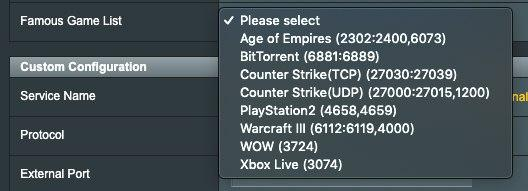
\includegraphics[width=.9\linewidth]{./assets/famous-games.jpg}
\caption{A router's configuration screen, showing a list of "famous games" including Bittorrent. From \href{https://twitter.com/tjhorner}{@tjhorner} on Twitter.}
\end{figure}
\end{frame}

\begin{frame}[label={sec:org14fc2bd}]{Security vulnerabilities}
  \note{Clearly, there are lots of opportunities for the software we run on our
    routers to face security vulnerabilities. However, when we're picking out
    our stack ourselves, we have the option to limit our risk by choosing a
    minimal set of tools-and updating quickly, or as quickly as our vendor can.}

  \begin{itemize}
  \item Insecure default passwords and configurations
    \note{There are insecure default settings on so many routers, and they often
      support management protocols which are also inherently insecure.}

  \item<2->{Out-of-date protocol stacks}
    \begin{itemize}
      \item<3-> WPAv3
      \item<4-> TLS 1.3
      \item<5-> SHA-1 deprecation
        \note{
          We don't \emph{use} SHA-1 any more, but I can guarantee there's a lot of
          equipment out there that still uses it, or even requires it
          }
    \end{itemize}
    
  \item<6-> Vendor security vulnerabilities
    \begin{itemize}
    \item<7-> Netgear routerlogin.net private cert
      \note {
        \href{https://gist.github.com/nstarke/a611a19aab433555e91c656fe1f030a9}{Netgear's routerlogin.net private cert} was found to have been leaked \emph{while I
          was writing this talk} and that's far from the only security issue we've
        seen.}

    \item<8-> Cisco NX-OS CVE-2020-3119
      \note{Turns out, Cisco's NX-OS' management protocol has a \href{https://nvd.nist.gov/vuln/detail/CVE-2020-3119}{stack overflow
          vulnerability}, which, combined with the OS' weak ASLR, lack of stack
        canaries, and the privileged context of the CDP parser means that a
        successful attack is devastating.}
    \end{itemize}
  \end{itemize}
\end{frame}

\subsection{Reasons to get your hands dirty}
\label{sec:org4ba3339}

\begin{frame}[label={sec:orgefe5704}]{Sheer edification}
\end{frame}

\begin{frame}[label={sec:org3f5e855}]{Complex systems encounter complex failures}
\note{
    Above a certain complexity, systems encounter emergent behaviors: unexpected
    and undesigned-for modes of operation that can manifest as failures and
    errors in ways that you may not understand. Actually building some
    familiarity with how networks work at a low level can help you comprehend
    what's happening when your systems fail.}

  \begin{figure}[htbp]
    \centering
    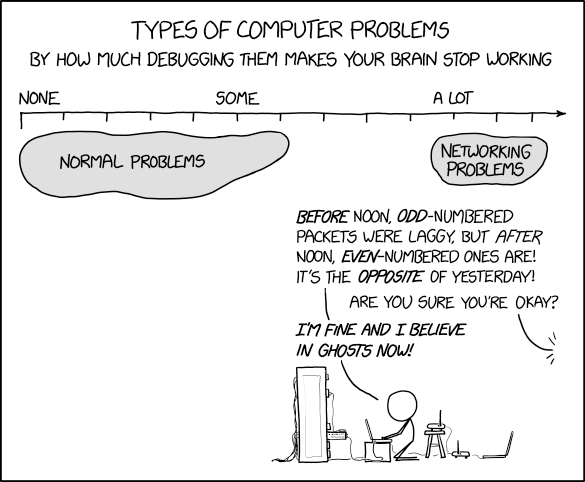
\includegraphics[width=.9\linewidth]{./assets/networking_problems.png}
    \caption{Take a bunch of complex systems and stick them together\ldots{} it'll be fine, right?}
  \end{figure}

\note{
    When building out a network, you're taking a bunch of complex systems, and
    by integrating all of them together, creating an even more complex
    meta-system. Debugging this system without context is difficult, to say the
    least, and you'll have more of a fighting chance with a deeper understanding
    of how a router actually operates-and what goes into network design.}
\end{frame}

\subsection{Goals for our router}
\label{sec:org778996d}

\begin{frame}[label={sec:org8d79961}]{Be upgradeable}
  \begin{itemize}
  \item Have expansion ports
  \item Support future enhancements
  \item Avoid getting trapped with insufficient hardware
  \end{itemize}
\note{While inexpensive, consumer routers are often extremely limited; if you look
at the OpenWRT wiki, there's an entire warning about 4/32 devices, which
have only 4MB of RAM and 32MB of flash storage; these devices can barely fit
their firmware when they're shipped out, let alone run extra tools! By using
commodity desktop hardware, we can swap out components, such as adding
higher-bandwidth NICs (10GbE hardware is pretty inexpensive now) or other
specialized additions.}
\end{frame}

\begin{frame}[label={sec:org1c4cf14}]{Be easy to manage}
\begin{block}{Familiar network analysis tools}
Instead of trying to figure out what strange configuration is present, or
divine what IP address has gotten assigned, all of your familiar command
line tools, like or are there, close at
hand.
\end{block}
\end{frame}

\begin{frame}[label={sec:org100ce9b}]{Be a test bed for exploring network ideas}
A full operating system on your router offers you lots of opportunities to
try out different tools or technologies

\begin{itemize}
  \item Docker containers on your router
    \note{I host my Unifi Controller on my router as a Docker container, which avoids
      using a separate physical device}

  \item<2-> Dynamic DNS
  \item<3-> A little home website
  \item<4-> Logging or traffic analysis
\end{itemize}
\end{frame}

\section{Selecting hardware}
\label{sec:org7a3497d}
\begin{frame}
  Selecting hardware
\note{
  I'm starting with hardware selection, but really both hardware and software
  have to be considered in tandem, since one will inform the other. This may
  evolve as you build your system, too! Maybe you decide that one approach isn't
  working for you after you've done some basic setup. That's okay. Just remember
  to take notes and log your progress.}
\end{frame}
\subsection{Constraints or parameters}
\label{sec:org9880863}
\note{
  Obviously, what capabilities you want to focus on will define how you select
  hardware to some extent; the short form is that as you want to have more
  capabilities captured in your router, you'll need more resources in general;
  there are some areas where you can optimize for a specific function.}

\begin{frame}[label={sec:org4c417ad}]{RAM}
4GB of RAM is more than enough for a basic firewall; if you want to add more
services, however, you'll want more. Once you start considering
virtualization, 16 or 32 might be needed or useful.
\end{frame}

\begin{frame}[label={sec:org5a31146}]{CPU}
Any recent CPU will be powerful enough--here your concerns are cost and
heat, mainly. Low-power embedded CPUs are great for low- or no-noise
operation. I do recommend multi-core, and if you'll be doing more crypto
on-board (TLS termination, VPN endpoint) your CPU should have SIMD
instructions.
\end{frame}

\begin{frame}[label={sec:org7599d13}]{Storage}
120GB SSDs are \$20 or less on Newegg; a lot of boards designed for a usecase
like this are also built to be booted off of flash drives or SD cards.

\begin{block}{Extra capacity}
If you're interested in doing more edge computing on your router-logging,
traffic shaping, running an HTTP server for a personal website (why not?)
you might want additional storage. This doesn't need to be an SSD, spinning
platters will do fine.
\end{block}
\end{frame}

\begin{frame}[label={sec:orgfdc6a4f}]{NICs}
  \note{
    This is the heart of choosing what you'll use as a router; at a minimum, you
    need two interfaces: one external, one internal. If you've got a separate
    switch you're using for your internal network, that may be all you need; if
    you want other machines directly connected to your router, however, you'll
    need more.}
  \begin{itemize}
  \item<2-3> Onboard, on-motherboard NICs
    \note{
      Assuming your motherboard has at least two NICs, you can forego all of the
      complexity and just use those devices.}

  \item<3> PCIe card NIC
    \note{
      If you want to do a little more than the motherboard can support directly,
      either in capacity or speed (or both!) an add-in card might be a good
      choice. With a PCIe card, you can get SFP+ ports and full 10GbE speeds.

      One issue I've encountered is, if you install an expansion card NIC, some
      motherboard firmwares will disable the onboard NIC by default. You may want
      that! In my case, I really didn't. So, if your NIC suddenly doesn't work when
      you install an additional one, you should look for this in the BIOS/EFI.}
  \end{itemize}

\begin{block}{Drivers a consideration}<4>
A key point with NIC selection is driver support; depending on your OS choice,
you may be more or less limited here! I recommend picking your NIC in
conjunction with your OS or after-so you can confirm what support you'll
have.
\end{block}

\begin{block}{Link Aggregation/Bonding and VLANs}<5>
You may encounter a situation where you want the core components of your
network to be on one subnet, and to have client devices on another; if
you've got a switch that can allocate ports to VLANs, then you can use one
larger, more capable switch to handle multiple subnets in parallel-but that
does require that your drivers support multiple VLANs on the same
connection, otherwise you'll need a separate connection from the router for
each subnet.
\end{block}

\begin{block}{Initial capacity requirement}<6>
When choosing a NIC for your build, you should keep your throughput
requirements in mind; if you host a media server inside your network, you
may want to have higher throughput on your LAN connection than your
WAN. Just try to keep your upstream and downstream in excess of what you'll
need for your connection.
\end{block}
\end{frame}

\subsection{Approaches}
\label{sec:org1558c43}

\begin{frame}[label={sec:org3e08734}]{Pre-built}
\note{Often slightly more expensive, but featureful systems. When looking at
    prebuilt equipment that runs pfSense or other similar firewall-oriented
    operating systems, you'll see purpose-built, but closer to commodity
    hardware than if buying from a vendor who builds a custom router OS like
    Ubiquiti or MikroTik.}

  \begin{itemize}
  \item QNAP
    \note{
      Mostly a NAS vendor, they have some switches and network equipment,
      including what they call a \href{https://www.qnap.com/en/product/qgd-1600p}{smart edge switch}, which looks a lot like what
      we're describing here.}

  \item<2-> Netgate firewalls
    \note{Ship with a pfSense license, this is great if you want an integrated
      solution.}
  \end{itemize}
\end{frame}

\begin{frame}[label={sec:org1e54b71}]{Small Form Factor}
\begin{block}{Standard desktop box}
Any relatively recent SFF desktop will do, as long as you can install the
parts you want to use in it!
\end{block}

\begin{block}{PCEngines APU units}
Useful boards for custom installations; if you're very space constrained or
have limited need for expandability, this might be a good choice.
\end{block}
\end{frame}

\begin{frame}[label={sec:org94796ed}]{Rackmount}
\begin{block}{Build your own}
Order parts from Supermicro, Tyan, other vendors, and build yourself a box!
This is a more expensive route, but can be very rewarding. If you're
building with Supermicro, do be aware that working in their cases can be a
little like kitbashing, and might involve some initially questionable
approaches. <Photos of my router build.>
\end{block}

\begin{block}{Buy used}
There's plenty of 1U servers with fantastic loadouts available for
relatively low prices. A manufacturer I was recently introduced to is HYVE,
who have some really cute boxes; they've got a focus on warm-temp
datacenters, and they're blue! <Photos of Duwamish>
\end{block}
\end{frame}

\subsection{Considerations for expandability}
\label{sec:org0ee9e3f}

\begin{frame}[label={sec:org2c89497}]{Future network standards}
\begin{block}{Gigabit now, what next?}
10 Gigabit hardware is getting really inexpensive! If you've got 8 PCIe gen 2
lanes available, you can have a dual SFP+ card. If you've got more, you can do
oh so much more. I've found multi-10-Gig/multi-gigabit cards, which can be handy
for virtualization down the line.
\end{block}

\begin{block}{Wireless upgrades}
If you get a wireless card that can run in AP mode, you can use your router as
your access point-and even trade out parts to upgrade to new standards as they
become available.
\end{block}
\end{frame}

\begin{frame}[label={sec:orgfcacbf9}]{Additional different hardware}
\begin{block}{Tensorflow PCIe!}
You can use Tensorflow in hardware now, relatively cheaply. They're \href{https://www.mouser.com/ProductDetail/Coral/G650-04527-01?qs=sGAEpiMZZMsG1k5vdNM\%252Fcyg9iDc\%25252Bz9JYkOSrS1TKoVU\%253D}{\$35 at
Mouser.} What would I do with these? I have no idea yet! But if you wanted to use
some tool like greylog to capture logs, you could run an ML model analysis on
it, and do so more efficiently than just on your CPU.
\end{block}

\begin{block}{TPM for security stuff}
While TPM support is limited generally, you can use it as a source of HWRNG, and
it can sometimes be used to offload cryptographic computations.
\end{block}
\end{frame}

\section{Software stack}
\label{sec:org2fd137a}
This is an area where there's lots of hot-headed opinions, and lots of options
without significant distinction. Decide what matters to you from the axes I'll
present, and remember that this choice is not permanent. You can try something,
decide it doesn't work, and change it out! That's okay!

\subsection{Axes of choice}
\label{sec:org84da425}

\begin{frame}[label={sec:orgb205e75}]{Interface style}
Some options are more configurable through webpages and graphical
environments, but are less configurable through text interfaces; careful
configuration of interfaces and potentially a VPN may be needed to remotely
manage some of these stacks.

For a more complete list to explore, check out \href{https://en.wikipedia.org/wiki/List\_of\_router\_and\_firewall\_distributions}{the list on Wikipedia}.

\begin{block}{Graphical/Web}
\begin{itemize}
\item pfSense
\item OPNsense
\item \href{https://www.clearos.com/}{clearOS}
\item \href{https://zeroshell.org/}{zeroshell}
\end{itemize}
\end{block}

\begin{block}{Textual}
\begin{itemize}
\item firewall-cmd (on any distro that supports it)
\item shorewall
\item \href{https://www.vyos.io/}{VyOS} - both free and paid, this one's complicated. Derivative of Brocade
Networks' OS.
\item raw nftables
\end{itemize}
\end{block}
\end{frame}

\begin{frame}[label={sec:orgdb902ba}]{Preference in base OS}
The mon0wall derivatives (pfSense, OPNsense) are all FreeBSD derivatives; in
other cases, you may prefer running a Linux kernel-for familiarity's sake,
or because of hardware support.
\end{frame}

\begin{frame}[label={sec:org991cbe7}]{Support model}
Paid support options exist for many firewall-oriented distros and
derivatives; generally speaking, there's also community support available,
but you may or may not find what you need in forums, especially when dealing
with unusual hardware or network configurations.
\end{frame}

\section{Configuring a router}
\label{sec:org2055775}
For our demo here, I'm going to use Fedora, and I'm going to configure it with
very low-level tools, to highlight fine details that graphical environments
might gloss over.

\subsection{Installing the OS}
\label{sec:orgfdf5a5f}
This part is probably the most ordinary aspect of this build. I'm going to use
Fedora Server, and I'm going to leave any graphical components out, while
making sure to set up SSH from the beginning.

\begin{frame}[fragile,label={sec:org98c7403}]{Important software to install before starting your journey}
 Before we start configuring components, it's a good idea to have a few tools
quick at hand.

\begin{block}{Text editor: \texttt{nano}}
I'm not normally a nano user, but it's got a very straightforward interface, and
all I really care about here is being able to edit files on the machine. I don't
care about having the most ergonomic environment for my daily driver needs.
\end{block}

\begin{block}{Terminal multiplexer: \texttt{tmux}}
Again, you may prefer other tools, but this is one I'm generally comfortable
with, and can usually get around in easily. If you're going to remote into your
machine a lot, you may want to configure it to be comfortable for you--but that
is not the goal of this exercise.
\end{block}
\end{frame}

\subsection{Configuring routing (for both IPv4 and IPv6)}
\label{sec:org5b3a27e}

\begin{frame}[label={sec:org8d7dd3d}]{Choose your network configuration tool}
NetworkManager, systemd-networkd are both viable options; here I'm using
systemd-networkd since it's what I've been using at home.

\begin{block}{Configure per-interface, per-file}
Configuration files will be applied in alphanumerical order, and later
configurations will override earlier ones; it's reasonable to have
baselines defined in low-numbered scripts, and more custom configurations
in high-numbered scripts. All network setups do this.
\end{block}


\begin{block}{Static or dynamic IP allocation}
\begin{block}{Static IP}
Useful for your gateway address on internal networks, or if you have a
static IP allocation from your ISP.
\end{block}

\begin{block}{Dynamic IP}
Handy when your upstream address is provided by DHCP; less handy if you're
trying to have routes declared statically.
\end{block}
\end{block}
\end{frame}

\begin{frame}[label={sec:org3a006ff}]{Multiple subnets and restricted routing}
\begin{block}{Non-routing subnet}
One useful configuration is to deliberately block IP forwarding on an
interface, to restrict the potential for devices (IoT in particular) to
leak information you might not want visible on the broader network. In this
case, you'd still run DHCP on the interface, but you would not present a
route to that network, and you would deliberately block forwarding for that
NIC.

Normally, to collect information from IoT devices that aren't routing to
the broader network, you need a dual-homed machine to collect logs or video
streams, for instance; when you're running a full Linux install on your
router, it \emph{is} a dual-homed machine, and can provide the access you
need. If you want to do more to limit your firewall's exposure, you might
consider a virtual machine; we'll talk about that in \ref{sec:org8517efe}.
\end{block}
\end{frame}

\subsection{Configuring IPv6 routing (Optional, recommended?)}
\label{sec:orgab512e8}

\begin{frame}[fragile,label={sec:orgf2a58cf}]{SLAAC and PD-assigned address}
 \begin{block}{accept\(_{\text{ra}}\) and the tri-state boolean}
From \href{https://www.kernel.org/doc/Documentation/networking/ip-sysctl.txt}{ip-sysctl.txt} in the Linux kernel documentation,
\begin{quote}
Possible values are:
    0 Do not accept Router Advertisements.
    1 Accept Router Advertisements if forwarding is disabled.
    2 Overrule forwarding behaviour. Accept Router Advertisements
      even if forwarding is enabled.
\end{quote}

Note that this means we'll want to set \texttt{accept\_ra} to \texttt{2} \emph{specifically} on our
WAN interface for IPv6 support.
\end{block}
\end{frame}

\begin{frame}[label={sec:orga4304bc}]{6to4 tunnel (Hurricane Electric)}
\end{frame}

\subsection{Configuring firewall rules}
\label{sec:org19a3785}

\begin{frame}[fragile,label={sec:org1530f3c}]{nftables versus frontends}
 Not really a "versus" here, but configuring nftables directly instead of using a
frontend is a viable path, and if you have custom logic for null-routing
specific IPs, you might want to have your own custom tooling writing your \texttt{.nft}
files and applying them. For this talk, we'll use firewalld. It's close to the
same syntax, but has some nice-to-have details like port numbers having service
names.
\end{frame}

\begin{frame}[label={sec:org9196245}]{Don't block ICMPv6!}
It's hard to stress this enough. Blocking ICMPv6 is a great way to cause
arbitrary, difficult-to-diagnose slowdowns if you have IPv6 support
enabled. This isn't going to improve your security posture, SLAAC with
security extensions will handle that.
\end{frame}

\begin{frame}[label={sec:org87a247f}]{Forwarding and NAT}
\end{frame}

\subsection{External services}
\label{sec:org55a4d52}

Part of the fun of running your own firewall is being able to host services on
it that would be limited or impossible on consumer hardware, and might be
difficult to configure on commercial hardware. Some of these can be quality of
life improvements (and may even be relatively straightforward to configure,
as some of them would need to exist inside your network as well.)

\begin{frame}[fragile,label={sec:org8635474}]{SSH}
 Being able to remotely connect to your firewall and check on the state of your
local network is useful--especially if you're away from home, and want to make
sure that a service is working. However, you'll want to take some precautions.

\begin{block}{Before enabling on your WAN interface}
\begin{block}{Disable password auth}
Add at least one public key to your user's authorized\(_{\text{keys}}\), validate that
you can connect with that key, then disable password authentication. Best
practices for SSH keys include using a different one on each device that
needs to connect, and potentially using a different key for each service
that you connect to with them. I recommend using \href{https://en.wikipedia.org/wiki/EdDSA\#Ed25519}{Ed25519} as the cipher;
it's short and powerful.
\end{block}
\begin{block}{Disable root login}
Most linux installs do this by default now, but it's always good to
check.
\end{block}
\end{block}

\begin{block}{When enabling on your WAN interface}
\begin{block}{Use a nonstandard port}
This is optional, but reduces the number of random drive-by attempts that
you'll see. I'm a fan of port 24. This can be done just with a firewall
rule, even!
\end{block}

\begin{block}{Consider fail2ban, logging}
In cases where you look at your \texttt{journalctl} logs and see lots of
attempted connections, you might consider adding fail2ban, and setting
some sufficiently high threshold--10 attempts, maybe. Remember when doing
this that it can bite \emph{you}, too.
\end{block}
\end{block}
\end{frame}

\begin{frame}[label={sec:org79d4237}]{Nice-to-have services}
\begin{block}{VPN}
Here we get into nice-to-have functionality, beyond the absolutely necessary. If
you want direct access to hosts inside your network from a remote location,
you'll want to use a VPN.

There's several approaches to this, largely depending on how willing you are to
DIY parts of the solution. Helpfully, \href{https://git.kernel.org/pub/scm/linux/kernel/git/torvalds/linux.git/commit/?id=bd2463ac7d7ec51d432f23bf0e893fb371a908cd}{Torvalds merged Wireguard into his branch
for 5.6}, so we should be able to rely on that being in production kernels soon,
and you won't need to install separate modules to get it working. There's a few
frontends for Wireguard under development now, but if you don't want to use
those there's OpenVPN, which is significantly more mature.
\end{block}

\begin{block}{Dynamic DNS}
Instead of memorizing your IP address, why not use a domain name? Services like
no-ip can offer you a way to get back to your own machines relatively easily,
but if you're willing to pay a little for a domain, there are plenty that are
very cheap--and then you just need to set up a script to auto-update your DNS
record regularly. Personally, I like Hurricane Electric for my DNS hosting
needs, but there's lots of options out there. Pick one you like, and have fun!
\end{block}

\begin{block}{Personal webpage}
Once you've got a domain name, clearly you need a website, too. Consider getting
a Let's Encrypt cert, while you're at it! Note that this is a fantastic service
to run in a container, or on another machine with port forwarding. If you take
the port forwarding route, just make sure to enable forwarding for as many ports
as you'll end up using--often both 80 and 443 are sufficient.
\end{block}
\end{frame}


\subsection{Debugging}
\label{sec:orgedb5cb4}

\begin{frame}[fragile,label={sec:orgba55011}]{Tools}
 All the tools you'd normally use to diagnose network connection issues
apply-layer 3 and above tools to determine inter-network connectivity like
\texttt{traceroute} and \texttt{ping}, but now we're also looking to understand firewall
issues like if DNS requests are being blocked, or even some layer 2 issues, like
whether or not our router's seeing ARP requests. This is where we start caring
about the difference between received packets and processed packets, and where
tools that interact directly with the NIC come in.

Some tools outside of the normal desktop network toolkit, then, that we'll want:
\begin{description}
\item[{tcpdump}] Collect logs directly from the firewall, on a given interface
\item[{Wireshark}] Collect and examine \emph{pcaps}, packet captures. Lets you
investigate failures at your leisure, and sift through captures
\end{description}

If these tools don't work on your router, you have a NIC that doesn't support
promiscuous mode (can pass through all packets, not just those for its MAC
address)-most should, but it's possible some won't. In that situation, you'll
need to find a different NIC to use if you want to be able to debug with these
tools.
\end{frame}

\begin{frame}[label={sec:org477961b}]{Classes of failure}
\begin{block}{Physical}
Sometimes cables go bad. Sometimes NICs are bad. When a NIC's bad, one often has
few options for recourse, but generally only a cable is bad. This might be as
trivial as one of the conductors failing, or it may be as strange as a cable
that's fine unless a specific frame goes through it. Bin the cable. Life's too
short for bad cables.
\end{block}

\begin{block}{Logical}
\begin{block}{Configuration error}
There's a great early-internet meme of the 500 mile email. Configuration
errors can happen to the best of us, and they will manifest in myriad
ways. Strange traffic patterns, machines that can't communicate with each
other, things which work outside the network not working inside\ldots{} you
name it!
\end{block}

\begin{block}{Assumption fault}
This is a fun one. Sometimes your logical error is not in software-it's in
how you think about the situation. An assumption fault can come up all
sorts of ways-routes that don't work, network segments not being
shared-but when they're encountered, diagramming them can help.
\end{block}
\end{block}
\end{frame}

\subsection{Recovery and fault-tolerance}
\label{sec:orgcb67d08}
Failures happen, unfortunately. Power outages strike, hard drives crash,
stray voltage kills your SSD's controller\ldots{}

\ldots{} and then you need to get into your router.

\begin{frame}[label={sec:orgbfa871a}]{Backups!}
Backing up key information matters a lot; this can be in the form of a
full-system backup, or as a build and design log. I'm a big fan of logging
my builds in markdown, or Org mode, or whatever journalling mechanism is
most convenient-then storing it in Git and keeping it off-site, on a service
like Gitlab, Bitbucket, or Gitlab.
\end{frame}

\begin{frame}[label={sec:org48c7f73}]{Break glass}
Maybe your only laptop with an SSH key for your router on it had a hard
drive failure, or you had a device stolen. In this case, if you can't get
into your router because you've properly locked it down, you're in a
pickle.

\begin{block}{IPMI or Serial Console access}
Assuming you have physical access to the server, you can connect a serial
console, and, assuming you've enabled it ahead of time for the machine, you
can sign in directly through that interface. If you have IPMI that supports
integrated KVM, such as a Supermicro machine or a suitably-licensed Dell or
HP board, you can do the same direct login.
\end{block}

\begin{block}{Spare private key}
Whether the private key is stashed in a password manager, on a USB stick,
or encoded in a QR code, having an extra public key provisioned on your
router, with the private key on a separate physical device allows you to
maintain access to the router, from any device with an SSH client, without
pre-provisioning it.

With this mechanism, especially if the key is stored in some sort of
off-site backup, you'll want to regenerate your break-glass key after
resolving your lack of access, and stash the new one in its place;
otherwise, your extra credential is now just another credential that you
can use from that or any machine.
\end{block}
\end{frame}

\section{Other configurations}
\label{sec:org319584b}

\subsection{Virtualized firewall}
\label{sec:org8517efe}

\begin{frame}[label={sec:org10a5a15}]{Why}
\begin{block}{Reducing risk from compromise}
Being the gateway device that has the most internet-facing surface area, your
firewall is a prime target for attack. By running the firewall as a virtual
machine instead of as the host, you can apply more restrictions to the
firewall than you could with it running as the main OS. Now, it can only
access storage or any other device that is assigned to it.
\end{block}

\begin{block}{Virtual firewall for virtual machines}
A common approach to securing multiple virtual services is to run a
firewall VM and have it act as the gateway for all of your virtual
machines, instead of having the host also operate as the gateway; this
approach allows you to have hidden services inside the network you've
created, and treat your virtual network as you would a physical
network.
\end{block}

\begin{block}{Quick update/deployment}
Updates to a virtual machine, depending on the approach, can be applied
extremely quickly and with little downtime.
\end{block}
\end{frame}

\begin{frame}[fragile,label={sec:org80a262d}]{How}
 \begin{block}{Pick your OS}
Basically all the questions we asked above apply twice, now; we need to
determine how much physical RAM our VM host needs, and of that amount, how much
the VM needs. A multi-core processor, and preferably with a lot of cores, is
essential.
\end{block}

\begin{block}{Connect your VM to the network}
\begin{block}{Bridging a physical NIC}
One common approach is to connect the VM to one of the host machine's NICs
through a sort of bridge.

\begin{block}{Linux Bridge interface}
One option is to make your host also route packets, although this might be said
to defeat the purpose of the firewall here.
\end{block}

\begin{block}{\href{https://en.wikipedia.org/wiki/Promiscuous\_mode}{Promiscuous Mode NIC}}
In this mode the NIC passes all packets it receives to the kernel, which means
it can respond to multiple MAC addresses if the host(s) so choose; this is a
common approach to allow one or multiple VMs to share a network connection with
a host.
\end{block}
\end{block}

\begin{block}{PCIe Passthrough NIC}
For my virtual firewall setup, i've opted to dedicate an entire physical card
with multiple ports to the firewall, and thereby made my VM host indirectly
connected to the main network. To achieve this I ended up adding an instruction
to load \texttt{pcistub} as the driver for a specific device to the kernel command
line.
\end{block}
\end{block}
\end{frame}

\begin{frame}[fragile,label={sec:org44af7c6}]{Issues you might run into}
 \begin{block}{Drivers and PCIe Passthrough}
I've been setting up an OPNsense VM to operate as the firewall for my
hackerspace; the server I purchased to function as our new firewall is far
more powerful than is necessary for a firewall alone, so I figured I'd host
some extra machines alongside the firewall, and get more use out of the
server.

Well, the Chelsio NIC I added to the server required a fair amount of
massaging to let me actually do the passthrough; I ended up needing to
use the \texttt{pcistub} kernel command line option for the whole card to stop the
kernel from loading the drivers for it.
\end{block}

\begin{block}{Virtual bridged network}
If you're using \texttt{virsh} to establish your networks, for a virtual network where
the firewall VM is the gateway, you'll need to specify how all your VMs attach
to it by configuring the network in their XML config to not have a forwarding
entry.
\end{block}
\end{frame}

\subsection{Multiple firewalls}
\label{sec:org5849af4}
Seen as a "defense in depth" strategy, this takes the medieval walled city
approach to network design. Here, we have potentially two levels of network;
we might want to keep "soft hosts"--personal computers, other relatively
unsecured systems--behind a more restricted firewall, while still allowing
machines operating as servers to have a more porous environment to work
in--potentially with other untrusted devices there as well (such as IoT
devices).

\subsection{Throughput considerations - Extension points}
\label{sec:orgb9c111a}

\begin{frame}[label={sec:org13ce3d4}]{Jumbo Frames}
The standard MTU is 1500B; this is fine in a reasonably fast network, but does
have a not-insignificant amount of overhead. That MTU includes the IP header,
after all, and especially on an IPv6 network, that can be quite large.

There's unfortunately issues with using DHCP to announce the MTU of a network;
many DHCP clients will simply ignore your stated value and use 1500, so until
jumbo frames in consumer OSes start showing up more often, we're going to have
to set this aside.
\end{frame}

\begin{frame}[label={sec:orgc8262cc}]{TCP offload}
An interesting technology but not widely supported; the primary vendor who's
pushing for this tech is Chelsio; they've \href{https://lwn.net/Articles/148697/}{attempted in the past} to get offload
support built into the Linux kernel, but were rebuked on the grounds that this
moves kernel decisions into a black box; we may yet see some changes in this
attitude, but it is generally outside the scope of this talk.
\end{frame}

\section{Lab}
\label{sec:org475924a}

Let's build a router real quick!

Set up a virtual firewall for other virtual hosts (mayyybe?)

For the purposes of this section, we'll focus on a minimal firewall setup that
covers the basic needs of a firewall, with clear extension points.

\subsection{Installing the OS}
\label{sec:org4390e2a}

\subsection{Setting up network configurations}
\label{sec:orgc20c062}

\begin{frame}[fragile,label={sec:org6f2d154}]{The \texttt{/proc/sys/net} filesystem and \texttt{/etc/sysctl.d}}
     This filesystem will tell you a lot about the configuration of your network,
    and the files in \texttt{/etc/sysctl.d} will set values at boot which can also be
    dynamically configured; files in this folder are read in sort order, which
    is why files are usually prefixed with a number denoting importance, low to
    high. An example of a line in one of these config files is as follows:
\#+NAME ipv4-conf-martians-example
\begin{verbatim}
net.ipv4.conf.all.log_martians = TRUE
\end{verbatim}

This line sets \texttt{/proc/sys/net/ipv4/conf/all/log\_martians} to \texttt{TRUE}; that will
log any and all impossible addresses received by the machine to the kernel
log. This could be useful if you're seeing a lot of unrouteable traffic on your
network, for instance.

\begin{block}{\texttt{forwarding}}
To set up forwarding with networkd, you'll want to include the following
block in a configuration file matching each interface you want to forward
traffic.

\#+NAME networkd-forwarding
\begin{verbatim}
[Network]
IPForward=yes
\end{verbatim}

For every interface that's going to be routing traffic, when you check
\texttt{/proc/sys/net/ipv4/conf/\$IFACE/forwarding} it should show \texttt{1}; for
non-forwarding interfaces, it'll show a \texttt{0}. (If it shows any non-zero
value, that's correct.
\end{block}

\begin{block}{Static IP configuration}
Declare your address and subnet with the following network block (you only
need one block with each ehading, but this is useful to differentiate.)

\#+NAME networkd-static-ip
\begin{verbatim}
[Network]
Address=172.24.3.1/24
\end{verbatim}
\end{block}

\begin{block}{Dynamic IP configuration (IPv4)}
Turning on DHCP is similarly straightforward.

\#+NAME netword-dhcp
\begin{verbatim}
[Network]
DHCP=ipv4
\end{verbatim}
\end{block}
\end{frame}

\begin{frame}[fragile,label={sec:orge0b857e}]{Setting MTU}
 \begin{block}{For the interface directly}
     We're using 9022 bytes here since that's large enough for various ethernet
     headers, and still gives us a full jumbo frame.
\#+NAME networkd-mtu
\begin{verbatim}
[Link]
MTUBytes=9022
\end{verbatim}
\end{block}

\begin{block}{For DHCP}
\end{block}
\end{frame}


\subsection{Setting firewall rules}
\label{sec:org6569745}

\begin{frame}[label={sec:org2862f08}]{Standard traffic rules}
\begin{block}{masquerade for IPv4}
\end{block}

\begin{block}{Restricting access for a given subnet}
As an extension of the concept of the \ref{sec:org0cc14b8} you can also
have the firewall deny connections from an IoT device subnet into your main
subnet or subnets.
\end{block}
\end{frame}

\begin{frame}[fragile,label={sec:orgc73d656}]{Port forwarding for services}
 This is a form of single-port, one-to-one NAT; with this forwarding, you
pick a single external port to surface on your public IP address and forward
it to a specific internal port on either the firewall or another internal
system. An example of this might be an internal web server:

\#+NAME firewalld-https-forward
\begin{verbatim}
# This also needs to be run in permanent mode, but the short demo works.
firewall-cmd --add-forward-port=port=80:proto=tcp:toport=80:toaddr=172.24.3.2
firewall-cmd --add-forward-port=port=443:proto=tcp:toport=443:toaddr=172.24.3.2
\end{verbatim}

With this port forwarded, our machine at \texttt{172.24.3.2} can now serve HTTP and
HTTPS content, and we can proceed to use (for example) Let's Encrypt to
secure it. Note that if you want to use a server on a different port to handle
getting that certificate, you'll need to add another exemption for it.
\end{frame}
\end{document}
